\documentclass[12pt,a4paper]{amsart}
% ukazi za delo s slovenscino -- izberi kodiranje, ki ti ustreza
\usepackage[slovene]{babel}
\usepackage[utf8]{inputenc}
\usepackage[T1]{fontenc}
\usepackage{multirow}
\usepackage{amsmath,amssymb,amsfonts}
\usepackage{url}
\usepackage[normalem]{ulem}
\usepackage[dvipsnames,usenames]{color}
\usepackage{csquotes}
\usepackage{caption}
\usepackage{lipsum}
\usepackage{hyperref}
\usepackage{tikz}
\usepackage{listings}
\usepackage{xcolor}
\usepackage{graphicx}
\usepackage{subcaption}


\lstset{
    breaklines=true,    
    breakatwhitespace=false,
    postbreak=\space,   
    tabsize=2,    
    basicstyle=\small\ttfamily\bfseries,
    commentstyle=\color{green!50!black},
    keywordstyle=\color{blue},
    numberstyle=\tiny\color{gray},
    numbers=left
}
\usetikzlibrary{graphs}
\usetikzlibrary{graphs.standard}

\makeatletter
\renewcommand\section{\@startsection{section}{1}%
  \z@{.5\linespacing\@plus.7\linespacing}{.5\linespacing}%
  {\normalfont\scshape\large\centering}}
\renewcommand\subsection{\@startsection{subsection}{2}%
  \z@{.5\linespacing\@plus.7\linespacing}{.5\linespacing}%
  {\normalfont\scshape}}
\renewcommand\subsubsection{\@startsection{subsubsection}{3}%
  \z@{.5\linespacing\@plus.7\linespacing}{-.5em}%
  {\normalfont\itshape}}
\makeatother

% ne spreminjaj podatkov, ki vplivajo na obliko strani
\textwidth 15cm
\textheight 24cm
\oddsidemargin.5cm
\evensidemargin.5cm
\topmargin-5mm
\addtolength{\footskip}{10pt}
\pagestyle{plain}
\overfullrule=15pt % oznaci predlogo vrstico


% ukazi za matematicna okolja
\theoremstyle{plain} % tekst napisan pokoncno
\newtheorem{definicija}{Definicija}[section]
\newtheorem{primer}[definicija]{Primer}
\newtheorem{definition}{Definicija}[section]

\renewcommand\endprimer{\hfill$\diamondsuit$}

% za stevilske mnozice uporabi naslednje simbole
\newcommand{\R}{\mathbb R}
\newcommand{\N}{\mathbb N}
\newcommand{\Z}{\mathbb Z}
\newcommand{\C}{\mathbb C}
\newcommand{\Q}{\mathbb Q}

% ukaz za slovarsko geslo
\newlength{\odstavek}
\setlength{\odstavek}{\parindent}
\newcommand{\geslo}[2]{\noindent\textbf{#1}\hspace*{3mm}\hangindent=\parindent\hangafter=1 #2}

% naslednje ukaze ustrezno popravi
\newcommand{\program}{Finančna matematika} % ime studijskega programa: Matematika/Finančna matematika
\newcommand{\imeavtorja}{Miha Jan, Sara Žužek} % ime avtorja
\newcommand{\imementorja}{doc. dr. Janoš Vidali} % akademski naziv in ime mentorja
\newcommand{\imesomentorja}{prof. dr. Riste Škrekovski}
\newcommand{\naslovdela}{Weak k-Metric Dimension}
\newcommand{\letnica}{2024} %letnica 


%%%%%%%%%%%%%%%%%%%%%%%%%%%%%%%%%%%%%%%%%%%%%%%%%%%%%%%%%%%%%%%%%%%%%%%%%%%%%%%%%%%%%%%%%%
\begin{document}

\thispagestyle{empty}
\noindent{\large
UNIVERZA V LJUBLJANI\\[1mm]
FAKULTETA ZA MATEMATIKO IN FIZIKO\\[5mm]
\program\ }
\vfill

\begin{center}{\large
\imeavtorja\\[2mm]
{\bf \naslovdela}\\[10mm]
Skupinski projekt\\[2mm]
Poročilo\\[1cm]
Mentorja: \imementorja, \\ \imesomentorja\\[2mm]}
\end{center}
\vfill

\noindent{\large
Ljubljana, januar \letnica}
\pagebreak

%%%%%%%%%%%%%%%%%%%%%%%%%%%%%%%%%%%%%%%%%%%%%%%%%%%%%%%%%%%%%%%%%
\section{Navodilo naloge}
Implement an ILP model for this invariant, and then write separate
small programs in Sage to answer each of following questions by exhaustive search.
\begin{enumerate}
    \item Find graphs for which $wdim_k(G) = \Delta(x, y)$ for a pair of vertices $x, y \in V(G)$ such that
    $d(x, y) \geq 3$.
    \item Determine $\kappa(G)$ and $wdim_k(G)$ for Cartesian products of cycles $G = C_a \square C_b$.
    \item  Determine the graphs G with $wdim_k(G) = dim_k(G)$ for various k with $k \leq \kappa(G)$.
\end{enumerate}
For small graphs, apply a systematic search; for larger ones, apply some stochastic search.
\bigskip
%%%%%%%%%%%%%%%%%%%%%%%%%%%%%%%%%%%%%%%%%%%%%%%%%%%%%%%%%%%%%%%%%
\section{Opis problema}
Najina projektna naloga se bo navezovala na k-te šibke dimenzije grafov. Projekt bova razdelila na več manjših delov.
Najprej bova napisala ustrezen CLP, potem pa ločila najino delo na 3 podnaloge, odvisno od zahtevanih pogojev, ki so opisani
v zgornjem navodilu naloge.

Najin cilj je, na podlagi testiranja oz. generiranja, ugotoviti, če za grafe, ki ustrezajo določenim 
pogojem veljajo kakšne posebne lastnosti. 
Za majhne vrednosti vozlišč se bova problema lotila s testiranjem na grafih, 
za večje pa bova uporabila metodo simulated annealing.
\bigskip
%%%%%%%%%%%%%%%%%%%%%%%%%%%%%%%%%%%%%%%%%%%%%%%%%%%%%%%%%%%%%%%%%
\section{Definicije}
Za lažje razumevanje, si najprej poglejmo par definicij.
\begin{definition}
    Naj bo $S \subseteq V(G)$ in $a, b \in V(G) \cup E(G)$. Definiramo $\Delta_S (a,b)$ kot vsoto razlik razdalj od $a$ in $b$ do vsakega vozlišča $S$. 
    Torej je $$\Delta_S (a,b) = \sum_{s \in S } |d(s,a) - d(s,b)|.$$
    Označimo $\Delta_{V(G)} (a,b) = \Delta (a,b)$.
\end{definition}

\begin{definition} 
    {\bf Šibka (vozliščna) k-metrična dimenzija} grafa $G$ $wdim_k(G)$, je kardinalnost/moč
    najmanjše množice vozlišč $S$ grafa $G$, tako da za vsak par vozlišč $x,y \in V(G)$ velja $\Delta_S (x,y) \geq k$.
\end{definition}

\begin{definition}
    Največja vrednost parametra $k,$ za katerega je šibka k-metrična dimenzija grafa G smiselno definirana označimo z $\kappa(G)$. 
\end{definition}

\begin{definition}
    {\bf K-metrična dimenzija} grafa $G$ $dim_k(G)$ je velikost najmanjše množice vozlišč $S$ grafa $G$, ki reši graf $G$ in ji rečemo k-rešljiva množica. 
    Za razliko od standardne metrične dimenzije ta zahteva, da vsak par vozlišč reši vsaj k vozlišč. K-metrična dimenzija se ujema z običajno dimenzijo, ko je $k = 1$.
\end{definition}
\bigskip
%%%%%%%%%%%%%%%%%%%%%%%%%%%%%%%%%%%%%%%%%%%%%%%%%%%%%%%%%%%%%%%%%
\section{Potek dela}
Za reševanje opisanega problema sva uporabila okolje Sage (SageMath) znotraj spletne platforme CoCalc. 
V nadaljevanju bova opisala in dodala kodo le od nekaterih funkcij, celotna koda s komentarji
se nahaja na GitHub repozitorju, prilagava tudi \href{https://github.com/mihajan/Weak-k-Metric-Dimension}{povezavo}.
\bigskip

\section{Majhni grafi}
Najprej sva se osredotočila na pisanje funkcije, ki s pomočjo ustreznega in učinkovitega CLP izračuna
k-to šibko dimnezijo. Funkcija sprejme graf G in število k, ter vrne vrednost šibke k-metrične dimenzije grafa
ob upoštevanju potrebnih pogojev.
\bigskip 
\begin{small}
    \begin{lstlisting}
    def CLP_weak_k_dim(g, k_value):
        p = MixedIntegerLinearProgram(maximization=False)
        x = p.new_variable(binary = True)
        p.set_objective(sum(x[v] for v in g))

        vertices = list(g.vertices())
        for va, vb in itertools.combinations(vertices, 2):
            expr = sum(abs(g.distance(va, vi) - g.distance(vb, vi)) * x[vi] for vi in g)
            p.add_constraint(expr >= k_value)
        sum_x = sum(x[vi] for vi in g)
        p.add_constraint(sum_x >= k_value)
        optimalna_resitev = p.solve()

        return optimalna_resitev
    \end{lstlisting}
\end{small}
\bigskip

Nato sva s pomočjo vgrajene metode \verb|distances_all_pairs| definirala funkcijo \verb|all_distances(graph)|, ki izračuna 
razdalje med vsemi pari vozlišč. 
Definirala sva še dve funkciji, ki jih bova potrebovala kasneje za reševanje najinih podnalog. 

Prva (\verb|delta(graph)|) izračuna $\triangle(x,y)$ za vse pare vozlišč in vrne izračunane vrednosti v slovarju,
druga (\verb|kappa(graph)|) pa izračuna vrednost $\kappa(G)$.

\begin{lstlisting}
    def delta(graph):
        dist = all_distances(graph)
        vertices = graph.vertices()
        delta_results = {}
        for x in vertices:
            for y in vertices:
                if x != y:
                    delta_xy = sum(abs(dist[s][x] - dist[s][y]) for s in vertices)
                    delta_results[(x, y)] = delta_xy
                else:
                    continue
        return delta_results
\end{lstlisting}

\begin{lstlisting}
    def kappa(graph):
        delta_results = delta(graph)
        min_delta = min(delta_results.values())
        return min_delta
\end{lstlisting}
\bigskip

\subsection{Prvi del naloge}
V prvem delu naloge sva morala poiskati grafe za katere velja, da je  $wdim_k(G) = \Delta(x, y)$, 
pri čemer je razdalja med dvema vozliščema $x$ in $y$ večja ali enaka 3. 

Definirala sva funkcijo \verb|ujemanje_1(graph)|, ki za izbrani graf poišče vse pare vozlišč, ki so med sabo oddaljeni za
3 ali več ter izračuna njihove $\triangle(x,y)$. Nato izračuna vse smislene šibke dimenzije za podani graf.
Funkcija vrne vrednosti True ali False odvisno od veljavnosti zgornje enačbe, tam kjer so ujemanja jih tudi shrani.

V nadaljevanju sva napisala algoritem s pomočjo katerega sva našla grafe, ki ustrezajo najinim pogojem. 
Napisani algoritem je z uporabo funkcije nauty geng generiral vse povezane grafe, ki imajo najmanj m in največ n 
vozlišč (vrednosti m in n sva poljubno spreminjala). Problem, ki se je pojavil je ta, da je algoritem za veliko
število vozlišč prepočasen in ne vrne vseh grafov, saj jih je preveč, da bi vse izpisal, zato sva napisala 
drug algoritem, ki izpusti določene grafe.
\bigskip

\subsection{Drugi del naloge}
V tem delu naloge morava določiti $\kappa(G)$ in $wdim_k(G)$ za kartezične produkte ciklov $G = C_a \square C_b$.

Definirala sva funkcijo, ki sprejme dimenziji ciklov a in b in izračuna njun kartezični produkt ter željeni vrednosti 
$\kappa(G)$ in $wdim_k(G)$.

Napisala sva še par algoritmov s pomočjo katerih sva testirala iskane stvari na grafih.
\bigskip

\subsection{Tretji del naloge}
Najprej sva definirala CLP, ki je podoben zgornjemu, le da namesto šibke k-te dimenzije izračuna k-to dimenzijo grafa.
Definirala sva tudi funkciji, ki izračunata $\triangle(x,y)$ in $\kappa(G)$. 

Definirala sva funkcijo, ki za izbrani graf preveri, kje pride do ujemanj k-te in šibke k-te dimenzije grafov,
funkcija vrne slovar, ključi slovarja so vrednosti k, za katere se dimenziji ujemata, vrednosti pa so enake k-ti oz. šibki k-ti dimenziji.
Napisala sva tudi algoritem, ki deluje podobno kot tisti pri prvem delu naloge, le da ta poleg grafa
izpiše še, katere k-te in k-te šibke dimenzije grafa se ujemajo.
Potem pa sva napisala tudi funkcijo, ki preveri ujemanja le za posebne primere grafov, kot so Petersenovi in hiperkocke.

\section{Ugotovitve}
\subsection{Prvi del naloge}
Ugotovila sva, da enakost za povezane grafe začne veljati šele pri grafih z vsaj osmimi vozlišči.
Tako sva dobila 8 grafov, ki imajo 8 vozlišč in ustrezajo danim pogojem. Opazila sva, da vsi ustrezni grafi vsebujejo
tudi cikle dolžine 3. Vseh povezanih grafov z 8 vozlišči je 11.117, kar pomeni, da je vsak 1400 tak, 
ki ustreza najinim pogojem, oziroma $0,07\%$ vseh grafov. Spodnja tabela prikazuje koliko je grafov z določenim številom povezav. 
Vidimo da imajo vsi med 10-15 povezav, ter da je aritmetična sredina 11,75, mediana pa 11.

\begin{table}[h]
    \begin{center}
      \begin{tabular}{l|c} % <-- Alignments: 1st column left, 2nd middle and 3rd right, with vertical lines in between
        \textbf{Število povezav} & \textbf{Število grafov} \\
        \hline
        10 & 2 \\
        11 & 3 \\
        12 & 1 \\
        14 & 1 \\
        15 & 1 \\
      \end{tabular}
    \end{center}
    \caption{Število povezav za grafe z 8 vozlišči}
    \label{tab:tabela1}
\end{table}

\bigskip
\begin{figure}[h]
    \centering
    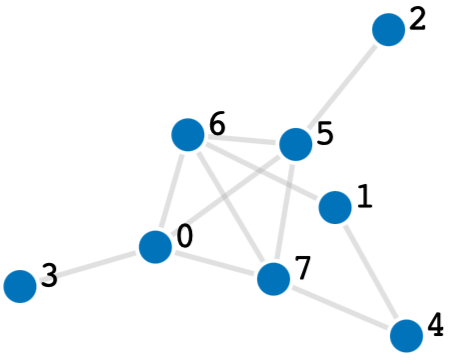
\includegraphics[width=0.25\textwidth]{graf1.png}
    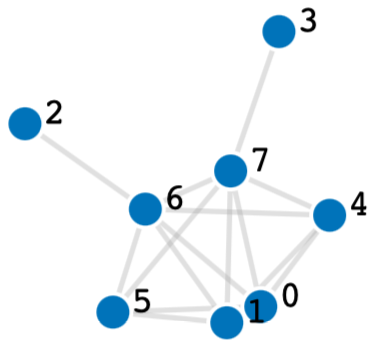
\includegraphics[width=0.25\textwidth]{graf2.png}
    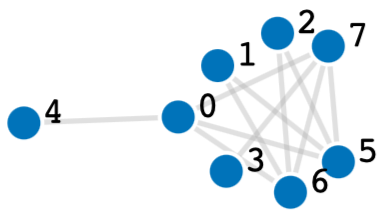
\includegraphics[width=0.25\textwidth]{graf3.png}
    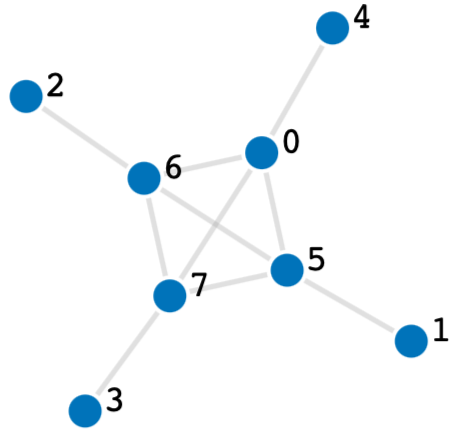
\includegraphics[width=0.25\textwidth]{graf4.png}
    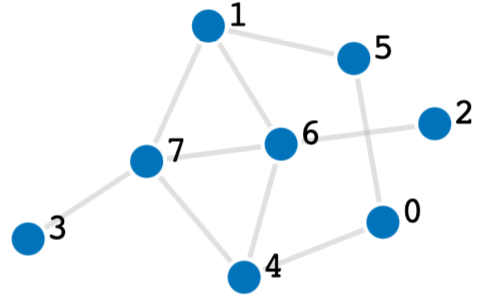
\includegraphics[width=0.25\textwidth]{graf5.png}
    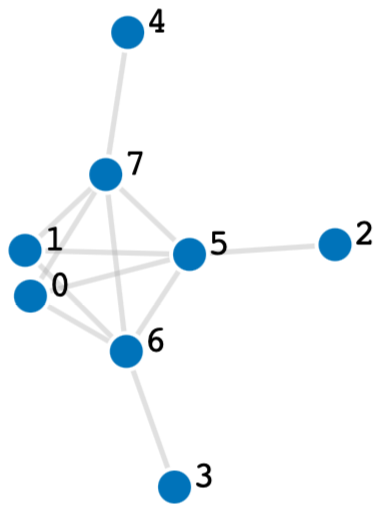
\includegraphics[width=0.25\textwidth]{graf6.png}
    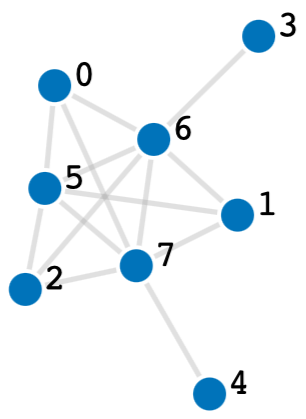
\includegraphics[width=0.2\textwidth]{graf7.png}
    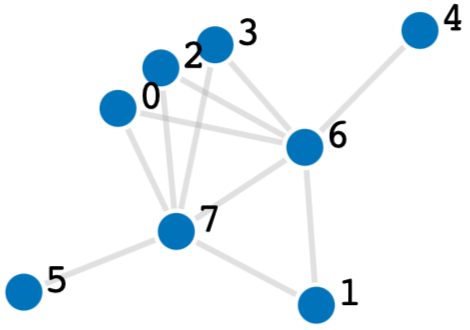
\includegraphics[width=0.25\textwidth]{graf8.png}
    \caption{Vsi grafi z osmimi vozlišči}
    \label{fig:slika1}
\end{figure}

Grafov z 9-mi vozlišči je mnogo več, celo tako veliko,
da program izpiše, da jih je preveč, da bi vse prikazal. Ker se število $\triangle(x,y)$ z naraščanjem vozlišč močno veča,
je več možnosti, da pride do enakosti z $wdim_k(G)$ in posledično je vedno več grafov, ki so ustrezni. Kot pričakovano, če 
večamo število vozlišč, dobimo vedno več grafov, ki ustrezajo pogojem, ne le po abosultni ampak tudi relativni spremembi.
Spodaj si poglejmo še dva primera grafov z več vozlišči. 
\bigskip

\bigskip

\bigskip
\begin{figure}[h]
    \centering
    \begin{subfigure}{0.25\textwidth}
    \centering
    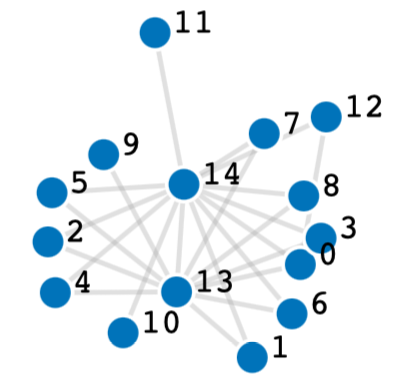
\includegraphics[width = \textwidth]{graf15.png}
    \end{subfigure}
    \begin{subfigure}{0.25\textwidth}
    \centering
    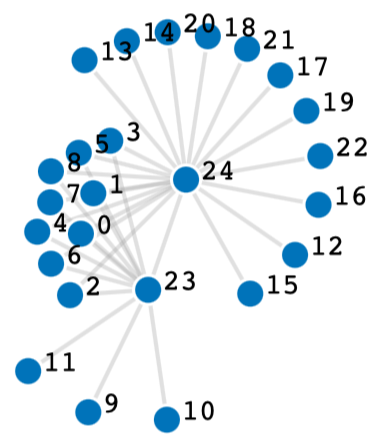
\includegraphics[width = \textwidth]{graf25.png}
    \end{subfigure}
    \caption{Primer grafa s 15 in 25 vozlišči}
    \label{fig:slika2}
\end{figure}%
    
\subsection{Drugi del naloge}
Vzemimo cikel A s številom vozlišč $a$ in cikel B s številom vozlišč $b$, njun kartezični produkt G ima število vozlišč $a \cdot b$. 
Na podlagi testiranja sva ugotovila, da velja formula za $\kappa(G)$ glede na to ali imata cikla A in B liho oziroma sodo število vozlišč. 
Medtem, ko je $wdim_k(G)$, če za $k$ vzamemo $\kappa(G)$ kar enaka $a \cdot b$.

Če imata oba cikla sodo število vozlišč, velja: $\kappa(G) = a \cdot b$.

Če imata oba liho število vozlišč, velja: $\kappa(G) = a \cdot b - max(a,b)$.

Če ima en liho in en sodo število vozlišč, pa velja: $\kappa(G) = a \cdot b - sodo(a,b)$.

\bigskip
\subsection{Tretji del naloge}
Pri povezanih grafih, generiranih s nauty geng, število ujemanj s številom vozlišč močno narašča.

Tako imamo za grafe s 4 vozlišči, 6 grafov, za katere velja $wdim_k(G) = dim_k(G)$.
Med njimi se trije ujemajo le za $k = 1$, preostali trije, pa se ujemajo za $k = 1,2$.

Medtem, ko je takih grafov, ki se ujemajo vsaj za en $k$ 21 s petimi vozlišči in 112 s šestimi vozlišči. 

\bigskip

Spodaj so prikazane slike vseh 6-ih grafov s štirimi vozlišči, ki imajo vsaj eno ujemanje.
\begin{figure}[h]
    \centering
    \includegraphics[width=0.22\textwidth]{naloga3_2_1.png}
    \includegraphics[width=0.17\textwidth]{naloga3_2_2.png}
    \includegraphics[width=0.22\textwidth]{naloga3_2_3.png}
    \caption{Grafi, ki se ujemajo za $wdim_1(G) = dim_1(G)$}
    \label{fig:slika1}
\end{figure}
\bigskip


\bigskip


\bigskip

\bigskip

\bigskip

\bigskip

\bigskip

\bigskip

\bigskip

\bigskip
\begin{figure}[h]
    \centering
    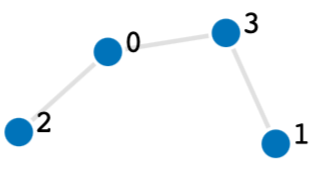
\includegraphics[width=0.22\textwidth]{naloga3_12.png}
    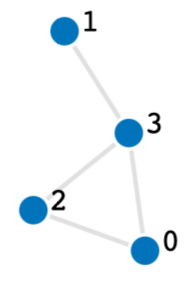
\includegraphics[width=0.17\textwidth]{naloga3_23.png}
    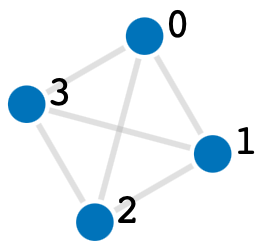
\includegraphics[width=0.17\textwidth]{naloga3_34.png}
    \caption{Grafi, ki se ujemajo za $wdim_k(G)=dim_k(G)$ za $k = 1,2$}
    \label{fig:slika1}
\end{figure}

\bigskip

Nato sva pogledala poseben primer grafov in sicer cikle.
Naj bo $n$ število vozlišč cikla, ugotovila sva, da se lihi cikli ujemajo za vse $k$ od $1$ do $n - 1$.
Sodi cikli pa se ujemajo le za $k = 1$. 

Testirala sva tudi za grafe, ki so kartezični produkti ciklov in ugotovila zanimivost, kjer imamo cikel A dolžine 3, cikel B 
pa je dolžine 6 ali več.

Velja, da se kartezični produkti oblike 3 x b, kjer je b sodo število, ujemajo za vse k, kjer je
$k = 1, 2, ... \kappa(G)$. Vrednosti za $wdim_k(G)=dim_k(G)$ naraščajo.

Za kartezične produkte 3 x b, kjer je b liho število pa je ujemanje enako kot za sode z izjemo 3 in 4.

\bigskip
Za Petersenove grafe nisva odkrila nobenega posebnega vzorca, ugotovila sva le, da se klasičen Peteresnov graf
ujema v vseh k-tih dimezijah.

\begin{figure}[h]
    \centering
    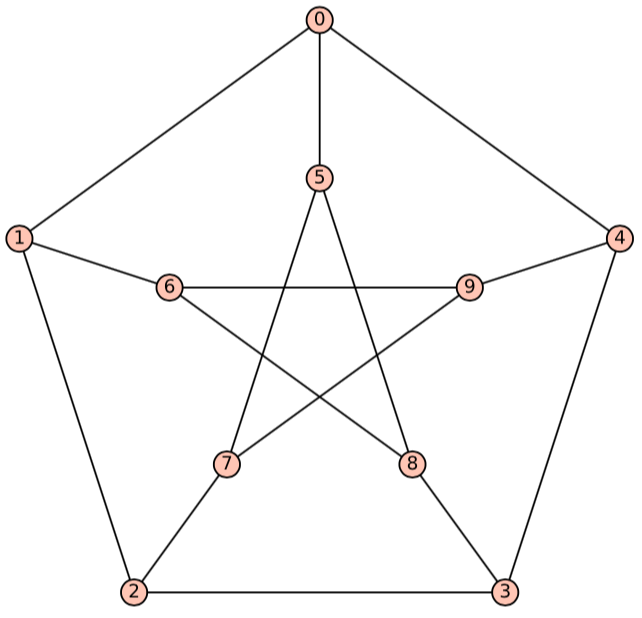
\includegraphics[width=0.35\textwidth]{petersen.png}
    \caption{Klasičen Petersenov graf}
    \label{fig:slika1}
\end{figure}


\section{Simulated annealing}
\end{document}